\chapter{Interview Transcript}

To further understand the processes of the current HRIS along with specific details, the researchers sent a formal interview request letter on July 1, 2024. The document has undergo-ed reviews, approval, and endorsement of the SP Adviser/Dean/CITO/CSIO, as well as the CCS Chairperson, and given that the project is an MIS initiative, the approval of the MIS Director is requested.

On July 5, 2024, the researchers conducted a formal interview along with the System Administrator Specialist, HRMO -- Ms. Leanne Gemelly B. Briones. The interview lasted from 3:00PM to 4:00PM.

The interview covered various aspects of the current HRMO system and processes, starting from a general overview regarding HRIS to user experience, system limitations, data management, current requirements, and diagrams and documents. This allowed the researchers to better gain understanding of the processes and identify priorities within modules to create and disregard.

\begin{figure}[H]
    \centering
    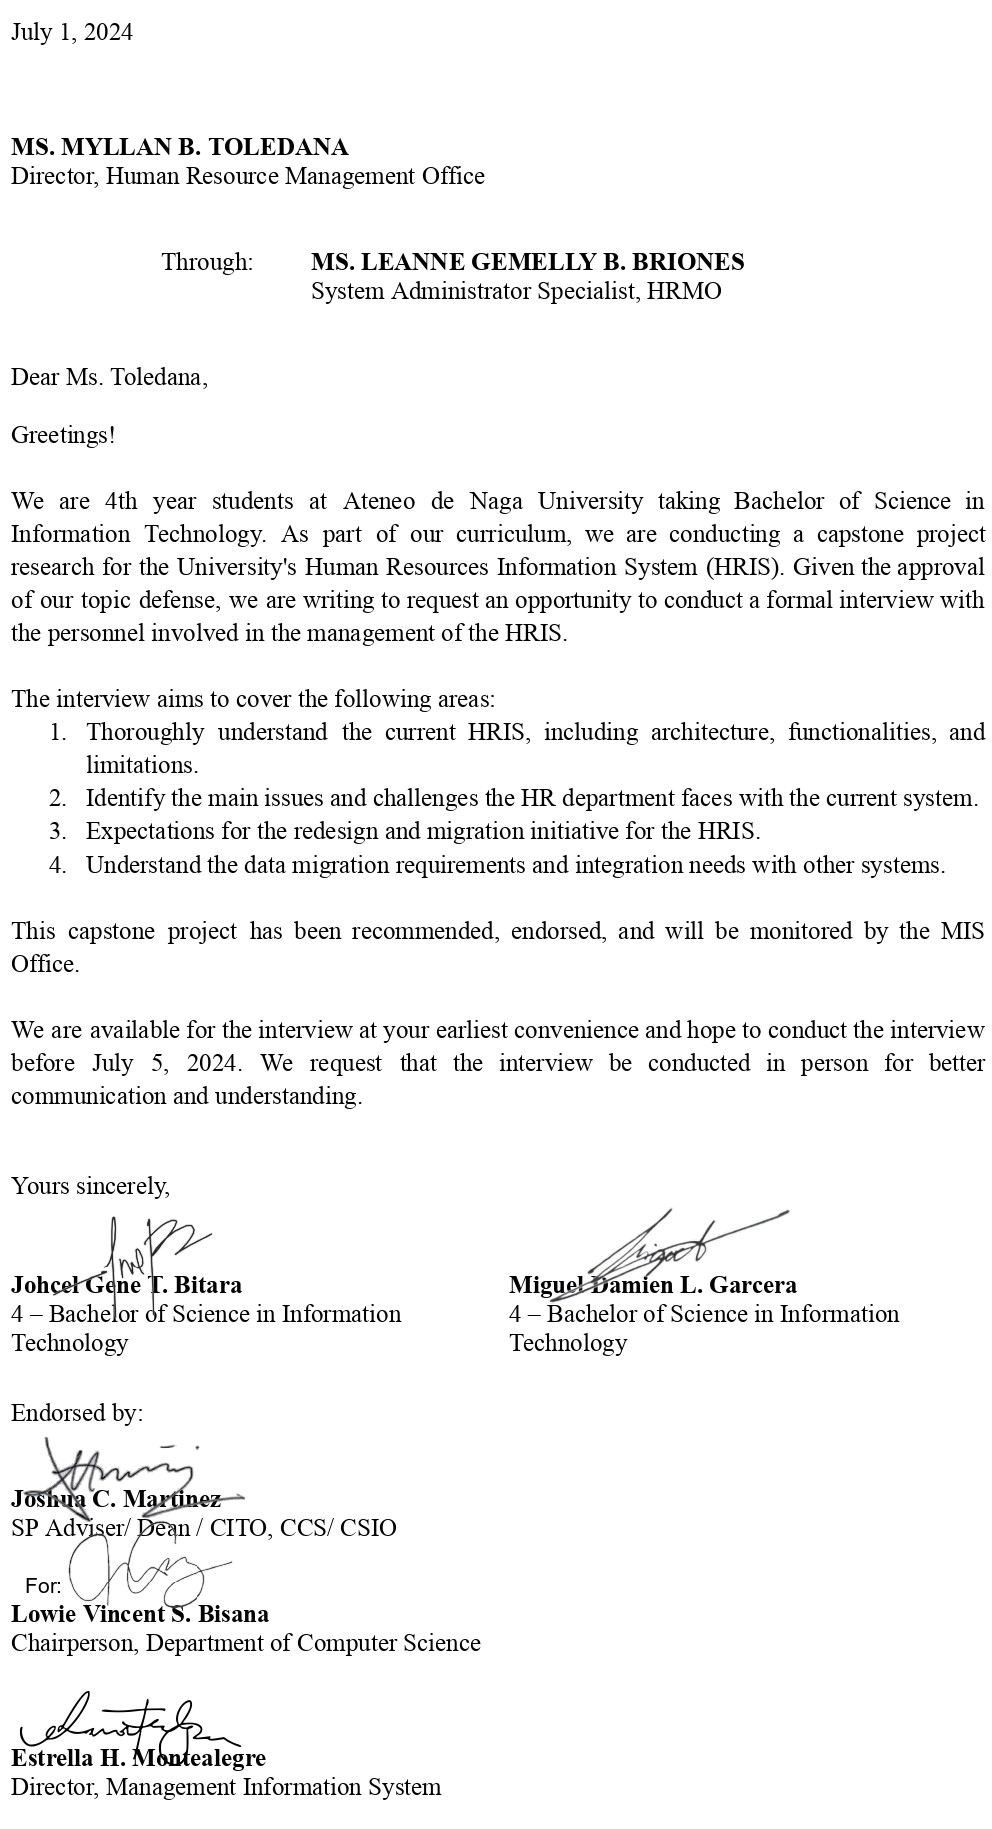
\includegraphics[width=.78\linewidth]{figures/misc/fig-interview-letter-request.jpg}
    \caption{Formal Interview Request.}
    \label{fig:enter-label}
\end{figure}

\begin{table}[H]
\begin{tabular}{@{}cll@{}}
\toprule
\multicolumn{1}{l}{} & \textbf{Modules}                         & \textbf{Brief Description}                                                            \\ \midrule
\textbf{HRIS MODULE} & Contacts                                 & Module use to save contact numbers within and outside the university                  \\
                     & Data Extraction                          & Module that handles query to retrieve processed information                           \\
                     & Personal Info                            & Module to store personal information of employees                                     \\
                     & General Employee Status Tracker          & Module use to track down status movements of the employees                            \\
                     & Employee Profile                         & Contains other information of the employees                                           \\
                     & Assignments                              & This module contains the active designation of the employee                           \\
                     & Assignment Archive                       & Contains the archived/history designation of the employees                            \\
                     & Faculty Rank                             & Modules that handles academic rank of the faculty                                     \\
                     & Academic Profile                         & Academic records of all employees                                                     \\
                     & Academic Awards                          & Module that handles the awards receive by the employee on a particular academic level \\
                     & Professional License Record              & Professional license record of employees                                              \\
                     & Training Attended Module                 & Contains record of training attended of employees                                     \\
                     & Performance Evaluation                   & Contains the average performance evaluation of each employee.                         \\
                     & COE                                      & Inputs the necessary data to produce the certificate of employment                    \\
                     & COE Reports                              & View of the newly requested COE                                                       \\
                     & Contracts/Appointment Generation Reports & Generates contracts/appointment of employees.                                         \\
                     & Health Record                            & Contains health info of the employee                                                  \\ \bottomrule
\end{tabular}
\end{table}

% \setspeaker{miguel}[Mr. Garcera]
% \setspeaker{hr}[Ms. Leanne]
% \setspeaker{gene}[Mr. Bitara]

% \addtolength{\transcriptlen}{4em}

% \begin{description}

%   \miguel I'm looking for a package to help with the layout of an interview transcript are there any good packages to do such a task. If possible could you provide a minimum working example?

%   \hr I'm looking for a package to help with the layout of an interview transcript are there any good packages to do such a task. If possible could you provide a minimum working example?

%   \gene Perhaps something that aligns the names to the text, and uses a columnar layout for the people vs what they said.

% \end{description}
